\chapter{Исследовательский раздел}
\label{cha:research}

В ходе выполнения дипломной работы было проведено исследование эффективности и применимости разработанного программного обеспечения, а также сделано сравнение результатов работы реализованного метода с результатами, полученными с помощью известных методов. Выявлены достоинства и недостатки разработанного программного комплекса.

\section{Способы оценки качества восстановленного изображения}

При сравнении изображений существуют различные методы и метрики, которые могут быть использованы для оценки их сходства или различия. Эти методы помогают количественно определить уровень сходства или несходства между изображениями, что может быть полезно в ряде приложений, таких как обработка изображений, компьютерное зрение и оценка качества.

\textbf{\textit{Пиковое отношение сигнал/шум (PSNR)}}--- это мера качества восстановленного изображения по сравнению с исходным\cite{metrics}. PSNR обычно используется для оценки эффективности алгоритмов обработки изображений и может быть рассчитан по следующей формуле:

\begin{equation}
    \text{PSNR} = 10 \log_{10} \frac{\text{MAX}_{i}^2}{\text{MSE}},
\end{equation}
где
\begin{itemize}
    \item $\text{PSNR}$ --- пиковое отношение сигнал/шум;
    \item $\text{MAX}_{i}$ --- максимально возможное значение пикселя изображения;
    \item $\text{MSE}$ --- средняя квадратичная ошибка между исходным и восстановленным изображением.
\end{itemize}

Средняя квадратичная ошибка определяется как:
\begin{equation}
    \text{MSE} = \frac{1}{mn} \sum_{i=1}^{m} \sum_{j=1}^{n} (I_{i,j} - I'_{i,j})^2,
\end{equation}
где
\begin{itemize}
    \item $m$ и $n$ --- размеры изображения;
    \item $I_{i,j}$ --- значение пикселя исходного изображения в позиции $(i,j)$;
    \item $I'_{i,j}$ --- значение пикселя восстановленного изображения в позиции $(i,j)$.
\end{itemize}

PSNR обычно выражается в децибелах (дБ) и рассчитывается по логарифмической шкале. Более высокое значение PSNR указывает на более высокое качество реконструкции, при этом максимально возможное значение составляет $\text{PSNR} = \infty$ для идеальной реконструкции. На практике значение PSNR 30 дБ или выше обычно считается хорошим качеством, в то время как значение ниже 20 дБ обычно считается плохим качеством.

PSNR --- полезная метрика для сравнения производительности различных алгоритмов обработки изображений, но у нее есть некоторые ограничения. Одно из этих ограничений заключается в том, что он не учитывает человеческое восприятие качества изображения, на которое могут влиять такие факторы, как пространственное распределение ошибок и наличие визуально заметных особенностей. В результате PSNR не всегда точно отражает субъективное качество изображения.

\textbf{\textit{Метрика структурного сходства изображений (SSIM)}} основана на идее  о том, что зрительная система человека обладает высокой адаптивностью и может мириться с некоторым ухудшением качества изображения при условии, что ухудшение не слишком сильное и общая структура изображения сохраняется \cite{metrics}. Для количественной оценки этой идеи индекс SSIM сравнивает яркость, контрастность и структуру двух изображений и объединяет эти сравнения в один балл.

Индекс SSIM определяется следующим образом:
\begin{equation}
    \text{SSIM}(x, y) = \frac{(2\mu_x\mu_y + c_1)(2\sigma_{xy} + c_2)}{(\mu_x^2 + \mu_y^2 + c_1)(\sigma_x^2 + \sigma_y^2 + c_2)},
\end{equation}
где
\begin{itemize}
    \item $x$ и $y$ --- два сравниваемых изображения;
    \item $\mu_x$ и $\mu_y$ --- средние значения пикселей в $x$ и $y$;
    \item $\sigma_x^2$ и $\sigma_y^2$ --- дисперсии значений пикселей в $x$ и $y$;
    \item $\sigma_{xy}$ --- ковариация значений пикселей в $x$ и $y$;
    \item $c_1$ и $c_2$ --- константы, используются для стабилизации разделения и обычно устанавливаются равными $c_1 = (0,01\cdot L)^2$ и $c_2 = (0,03\cdot L)^2$, величина $L$ описывает динамический диапазон значений пикселей.
\end{itemize}

Индекс SSIM варьируется от $-1$ до $1$, причем более высокие значения указывают на большее сходство между двумя изображениями.

\section{Описание данных для исследования}

Для исследования эффективности и применимости разработанного программного обеспечения будут использованы несколько произвольных изображений из тренировочного набора данных SIDD, описанного ранее. Помимо этого, будет использован набор данных RENOIR, аналогичный SIDD \cite{renoir}. 

Представленные наборы данных используют формат изображений без сжатия, поэтому изображения также переформатированы в формат JPEG для дополнительных исследований применимости разработанного ПО.

\section{Результаты работы программы}

Наряду с реализованным методом фильтрации в сравнении были представлены следующие методы устранения шумов на изображениях:
\begin{itemize}
    \item метод среднего;
    \item метод фильтрации по Гауссу;
    \item метод медианной фильтрации;
    \item метод билатеральной фильтрации;
    \item нейронная сеть ScuNet \cite{scunet}.
\end{itemize}

Используются следующие условные обозначения:
\begin{itemize}
    \item Ideal соответствует идеальному изображению без помех;
    \item Noised соответствует изображению с помехами;
    \item Mean соответствует фильтрации методом среднего;
    \item Gaussian соответствует методу фильтрации по Гауссу;
    \item Median соответствует методу медианной фильтрации;
    \item Bilateral соответствует методу билатеральной фильтрации;
    \item ScuNet соответствует фильтрации с использованием ScuNet;
    \item MyMethod соответствует фильтрации с использованием разработанного метода.
\end{itemize}

В таблицах \ref{tabular:sidd_results} и \ref{tabular:renoir_results} представлены усредненные величины метрик PSNR и SSIM, полученные на выборках SIDD и RENOIR соответственно.

\begin{table}[h!]
	\centering
    \captionsetup{justification=raggedleft,singlelinecheck=false}
	\caption{\label{tabular:sidd_results} Сравнительная таблица методов фильтрации шумов на изображениях набора данных SIDD}
	\begin{tabular}{|c|c|c|c|c|c|c|}
    \hline
    \textbf{Метрика} & \textbf{Mean} & \textbf{Gaussian} & \textbf{Median} & \textbf{Bilateral} & \textbf{ScuNet} & \textbf{MyMethod} \\ \hline
    PSNR & 28.553 & 28.982 & 29.401 & 29.653 & 33.071 & 33.393 \\ \hline
    SSIM & 0.693 & 0.697 & 0.707 & 0.755 & 0.905 & 0.917 \\ \hline
    \end{tabular}
\end{table}

\begin{table}[h!]
	\centering
    \captionsetup{justification=raggedleft,singlelinecheck=false}
	\caption{\label{tabular:renoir_results} Сравнительная таблица методов фильтрации шумов на изображениях набора данных RENOIR}
	\begin{tabular}{|c|c|c|c|c|c|c|}
    \hline
    \textbf{Метрика} & \textbf{Mean} & \textbf{Gaussian} & \textbf{Median} & \textbf{Bilateral} & \textbf{ScuNet} & \textbf{MyMethod} \\ \hline
    PSNR & 28.362 & 28.832 & 28.125 & 29.783 & 33.314 & 33.032 \\ \hline
    SSIM & 0.711 & 0.710 & 0.721 & 0.735 & 0.921 & 0.893 \\ \hline
    \end{tabular}
\end{table}

Исходя из количественных величин метрик можно сделать о том, что реализованный метод показывает сопоставимые результаты с нейронной сетью ScuNet и превосходит оставшиеся методы.

Для наиболее эффективных методов устранения помех: разработанного метода и ScuNet, было выполнено сравнение времени выполнения для изображений различного размера. Разработанный метод является более эффективным по времени выполнения.

\begin{table}[h!]
	\centering
    \captionsetup{justification=raggedleft,singlelinecheck=false}
	\caption{\label{tabular:renoir_results} Сравнительная таблица времени выполнения ScuNet и разработанного метода для изображений различного размера}
    \begin{tabular}{|c|c|c|c|}
    \hline
    Алгоритм & 256x256 & 512x512 & 1024x1024 \\ \hline
    ScuNet & 1.43 c & 6.38 c & 22.21 c \\ \hline
    MyMethod & 1.08 с & 4.46 c & 15.42 c \\ \hline
    \end{tabular}
\end{table}

Также следует произвести визуальную оценку полученных изображений, поскольку рассмотренные метрики не учитывают особенности восприятия человеческого глаза.

На рисунке \ref{fig:simple} представлены результаты работы алгоритмов устранения шумов на примере простого изображения.

На рисунке \ref{fig:complex} представлены результаты работы алгоритмов устранения шумов на примере сложного изображения. Нейронные сети показывают сопоставимый результат, следует отметить, что при высокой степени устранения шумов удалось сохранить четкие грани объектов и множество деталей.

На рисунке \ref{fig:format} представлены результаты работы алгоритмов на одном и том же изображении при использовании разных форматов хранения: PNG и JPG соответственно. В разработанном методе появляются артефакты при работе со сжатым изображением.

\begin{figure}
  \centering
  \begin{tabular}{cc}
    \begin{subfigure}{0.3\textwidth}
      
\includegraphics[width=\linewidth]{inc/research/simple/original.png}
      \caption{Ideal}
    \end{subfigure} &
    \begin{subfigure}{0.3\textwidth}
      
\includegraphics[width=\linewidth]{inc/research/simple/noised.png}
      \caption{Noised}
    \end{subfigure} \\
    
    \begin{subfigure}{0.3\textwidth}
      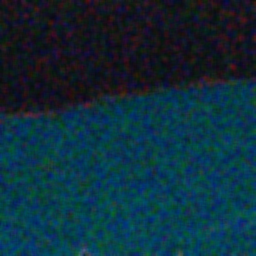
\includegraphics[width=\linewidth]{inc/research/simple/denoised_mean.png}
      \caption{Mean}
    \end{subfigure} &
    \begin{subfigure}{0.3\textwidth}
      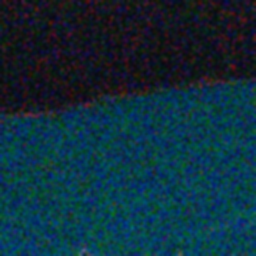
\includegraphics[width=\linewidth]{inc/research/simple/denoised_gaussian.png}
      \caption{Gaussian}
    \end{subfigure} \\
    
    \begin{subfigure}{0.3\textwidth}
      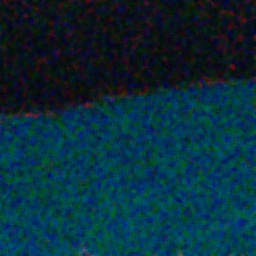
\includegraphics[width=\linewidth]{inc/research/simple/denoised_median.png}
      \caption{Median}
    \end{subfigure} &
    \begin{subfigure}{0.3\textwidth}
      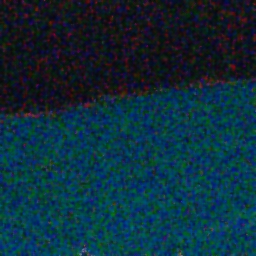
\includegraphics[width=\linewidth]{inc/research/simple/denoised_bilateral.png}
      \caption{Bilateral}
    \end{subfigure} \\
    
    \begin{subfigure}{0.3\textwidth}
      
\includegraphics[width=\linewidth]{inc/research/simple/denoised_scunet.png}
      \caption{ScuNet}
    \end{subfigure} &
    \begin{subfigure}{0.3\textwidth}
      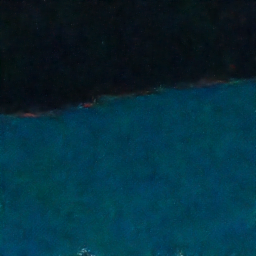
\includegraphics[width=\linewidth]{inc/research/simple/denoised_mycnn.png}
      \caption{MyMethod}
    \end{subfigure} \\
  \end{tabular}
  \caption{Сравнение алгоритмов на изображении с примитивной структурой и реальными шумами}
  \label{fig:simple}
\end{figure}

\begin{figure}
  \centering
  \begin{tabular}{cc}
    \begin{subfigure}{0.3\textwidth}
      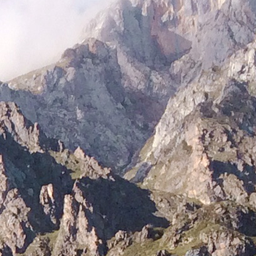
\includegraphics[width=\linewidth]{inc/research/complex/original.png}
      \caption{Ideal}
    \end{subfigure} &
    \begin{subfigure}{0.3\textwidth}
      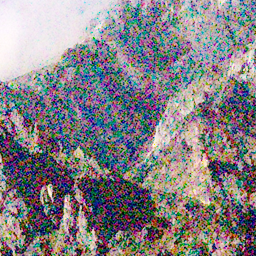
\includegraphics[width=\linewidth]{inc/research/complex/noised.png}
      \caption{Noised}
    \end{subfigure} \\
    
    \begin{subfigure}{0.3\textwidth}
      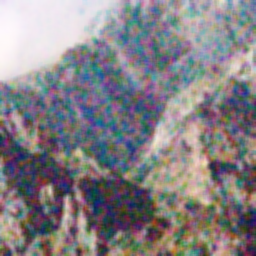
\includegraphics[width=\linewidth]{inc/research/complex/denoised_mean.png}
      \caption{Mean}
    \end{subfigure} &
    \begin{subfigure}{0.3\textwidth}
      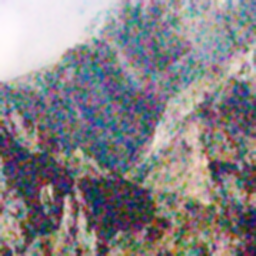
\includegraphics[width=\linewidth]{inc/research/complex/denoised_gaussian.png}
      \caption{Gaussian}
    \end{subfigure} \\
    
    \begin{subfigure}{0.3\textwidth}
      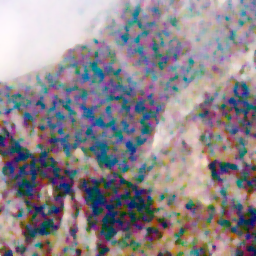
\includegraphics[width=\linewidth]{inc/research/complex/denoised_median.png}
      \caption{Median}
    \end{subfigure} &
    \begin{subfigure}{0.3\textwidth}
      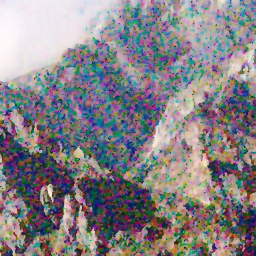
\includegraphics[width=\linewidth]{inc/research/complex/denoised_bilateral.png}
      \caption{Bilateral}
    \end{subfigure} \\
    
    \begin{subfigure}{0.3\textwidth}
      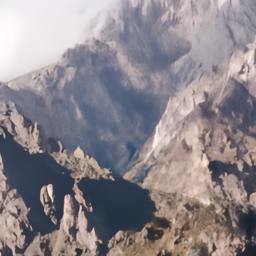
\includegraphics[width=\linewidth]{inc/research/complex/denoised_scunet.png}
      \caption{ScuNet}
    \end{subfigure} &
    \begin{subfigure}{0.3\textwidth}
      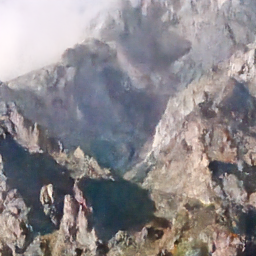
\includegraphics[width=\linewidth]{inc/research/complex/denoised_mycnn.png}
      \caption{MyMethod}
    \end{subfigure} \\
  \end{tabular}
  \caption{Сравнение алгоритмов на изображении со сложной структурой и реальными шумами}
  \label{fig:complex}
\end{figure}

\noindent
\begin{figure}
  \centering
  \begin{tabular}{cc}
    \begin{subfigure}{0.3\textwidth}
      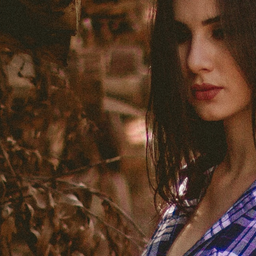
\includegraphics[width=\linewidth]{inc/research/formats/original_png.png}
      \caption{Ideal(PNG)}
    \end{subfigure} &
    \begin{subfigure}{0.3\textwidth}
      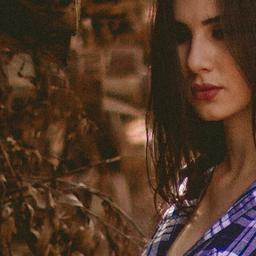
\includegraphics[width=\linewidth]{inc/research/formats/original_jpg.png}
      \caption{Ideal(JPG)}
    \end{subfigure} \\
    
    \begin{subfigure}{0.3\textwidth}
      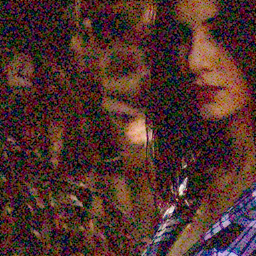
\includegraphics[width=\linewidth]{inc/research/formats/noised_png.png}
      \caption{Noised(PNG)}
    \end{subfigure} &
    \begin{subfigure}{0.3\textwidth}
      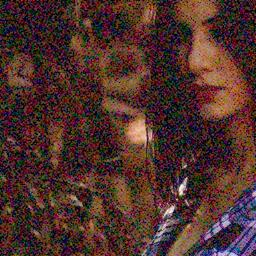
\includegraphics[width=\linewidth]{inc/research/formats/noised_jpg.png}
      \caption{Noised(JPG)}
    \end{subfigure} \\
    
    \begin{subfigure}{0.3\textwidth}
      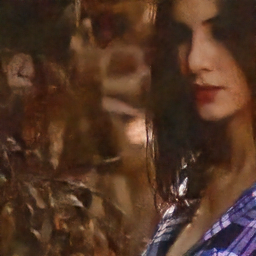
\includegraphics[width=\linewidth]{inc/research/formats/denoised_mycnn_png.png}
      \caption{MyMethod(PNG)}
    \end{subfigure} &
    \begin{subfigure}{0.3\textwidth}
      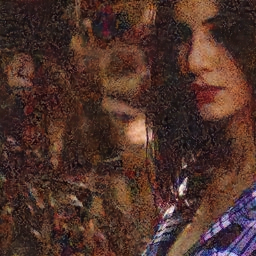
\includegraphics[width=\linewidth]{inc/research/formats/denoised_mycnn_jpg.png}
      \caption{MyMethod(JPG)}
    \end{subfigure} \\
    
    \begin{subfigure}{0.3\textwidth}
      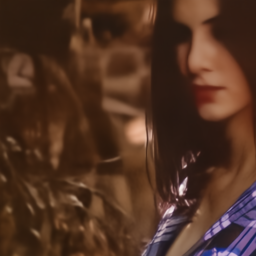
\includegraphics[width=\linewidth]{inc/research/formats/denoised_scunet_png.png}
      \caption{ScuNet(PNG)}
    \end{subfigure} &
    \begin{subfigure}{0.3\textwidth}
      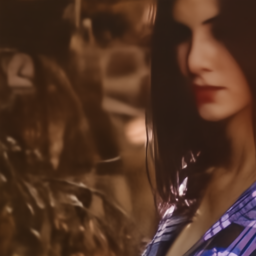
\includegraphics[width=\linewidth]{inc/research/formats/denoised_scunet_jpg.png}
      \caption{Scunet(JPG)}
    \end{subfigure} \\
  \end{tabular}
  \caption{Сравнение алгоритмов на изображении в форматах со сжатием и без сжатия, JPG и PNG соответственно}
  \label{fig:format}
\end{figure}

\section{Оценка разработанного программного комплекса}

Основываясь на результатах проведенных исследований программного комплекса, были выявлены описанные далее достоинства и недостатки.

Среди преимуществ разработанного ПО следует отметить:
\begin{itemize}
    \item работа с реальными шумами;
    \item высокая степень сохранения деталей изображения.
\end{itemize}

Также спроектированный метод нуждается в доработке в следующем аспекте:
\begin{itemize}
    \item форматы входных данных --- в форматах изображений, использующих сжатие для хранения, наблюдается ухудшение качества работы.
\end{itemize}

\newpage

\section{Выводы}

Было проведено исследование эффективности и применимости разработанного программного обеспечения, а также выполнено сравнение результатов работы реализованного метода с результатами, полученными с помощью известных методов. Выявлены достоинства и недостатки разработанного метода фильтрации малоразмерных шумов на цветных изображениях с помощью сверточных нейронных сетей.